%
% Szakdolgozatminta az Eszterházy Károly Katolikus Egyetem
% matematika illetve informatika szakos hallgatóinak.
%

\documentclass[
% opciók nélkül: egyoldalas nyomtatás, elektronikus verzió
% twoside,     % kétoldalas nyomtatás
% tocnopagenum,% oldalszámozás a tartalomjegyzék után kezdődik
]{thesis-ekf}
\usepackage[T1]{fontenc}
\PassOptionsToPackage{defaults=hu-min}{magyar.ldf}
\usepackage[magyar]{babel}
\usepackage{mathtools,amssymb,amsthm,pdfpages}
\footnotestyle{rule=fourth}

\newtheorem{tetel}{Tétel}[chapter]
\theoremstyle{definition}
\newtheorem{definicio}[tetel]{Definíció}
\theoremstyle{remark}
\newtheorem{megjegyzes}[tetel]{Megjegyzés}

\begin{document}

\institute{Matematikai és Informatikai Intézet}
\title{A szakdolgozat címe}
\author{Herbák Marcell\\Programtervező Informatikus BSc}
\supervisor{Dr. Kovásznai Gergely\\Egyetemi docens}
\city{Eger}
\date{2025}
\maketitle

\tableofcontents

\chapter{Bevezetés}

\section{Játék ismertetése}

\subsection{Játék ötlete}

\subsection{Játék szabályok}

A játék egy fixált méretű, négyzetekből álló, 7x10 nagyságú tábla. A játékot kettő játékos tudja játszani, melyből a szakdolgozatomban az egyik játékos a mesterséges intelligencia lesz. Mindegyik játékos rendelkezik karakterekkel, amelynek kezdő mennyisége a játék indítása előtt kiválasztható. Mindkét játékos rendelkezik minimum 1, maximum pedig 3 karakterrel. A karakterek mennyisége játékosonként eltérő lehet, nem szükséges mindkét játékosnak ugyanazzal a karakter mennyiséggel kezdenie. Az egyik játékos karakterei (több karakter esetén függőlegesen egy mező kihagyással) a 2. oszlopban, a másik játékos karakterei pedig a 9. oszlopban kezdenek. A karakterek rendelkeznek életerővel, minden karakter a játék kezdésekor 10 életerőponttal kezd. A táblán léteznek akadályozó mezők, amelyekre a játékosok nem léphetnek, illetve nem támadhatják meg.

A játék során a játékosok egymás után jönnek, egy körben az összes karakterükkel végre kell hajtaniuk egy interakciót. Ez a két interakció lehet:
\begin{itemize}
	\item Lépés
	\item Támadás
\end{itemize}
Lépés során a karakterükkel egy mezőt léphetnek a négy irány közül valamelyik irányba: fel, le, balra vagy jobbra. A játékos karaktere nem léphet olyan mezőre, amelyen már áll egy másik saját karakter, egy ellenfél karakter vagy egy akadály. Támadás során a játékos egy mezőn belül támadhat négy irány közül valamelyik irányba. A játékos karaktere nem támadhatja meg a saját karakterét, illetve nem támadhat üres vagy akadály mezőt. Támadás során a megtámadott karakter elveszít 1 életerő pontot. Amennyiben a játékos minden karakterére végrehajtott egy interakciót, a játékos átadja a körét a másik játékosnak.

Egy karakter, amennyiben elveszíti összes életerejét, eltűnik a tábláról, mezője felszabadul, illetve innentől kezdve azzal nem tud a játékos interakciót végrehajtani és nem hozhatja vissza.
 
A játékos célja, hogy ellenfele összes karakterét eltüntesse a tábláról. A játékot az a játékos nyeri, akinek marad legalább 1 karaktere a táblán, legalább 1 életerővel.

\chapter{Mesterséges intelligencia}

\section{Története}

\section{Minimax algoritmus}

\subsection{Minimax alfa-béta vágással}

\chapter{Technológiák}

\section{Játékmotor}

A szakdolgozatom megvalósításához a Unity-t (korábban Unity3D) használom. A Unity egy világszerte ismert és használt videójáték-motor, amelyet a Unity Technologies fejleszt 2005 óta. A motor támogat több különböző platformot, például PC, videójáték konzolok és okostelefonok. Különösen kedvelik a kezdő játékfejlesztők a letisztult felülete és egyszerű használata miatt. Választásom azért esett a Unity-re, mert a szkriptekhez natívan támogatja a C\# nyelvet. A szakdolgozatomban a Unity-nek a 2022.3.32f1-es verzióját használom.

\section{Grafikus szerkesztő}

\chapter{Implementáció}

\section{Játék megvalósítása}

\subsection{Állapottér}

\subsection{Operátor}

\subsection{Operátorok felépítése}

\subsection{Operátor generálás}

\subsection{Minimax}

\subsection{Minimax alfa-béta vágással}

\subsection{Heurisztika}

\subsection{Megjelenítés}


\chapter{Tesztelés}

\chapter*{Összegzés}
\addcontentsline{toc}{chapter}{Összegzés}


\begin{thebibliography}{2}
\addcontentsline{toc}{chapter}{\bibname}
\end{thebibliography}

% Aláírt, szkennelt nyilatkozat beillesztése a szakdolgozat végére
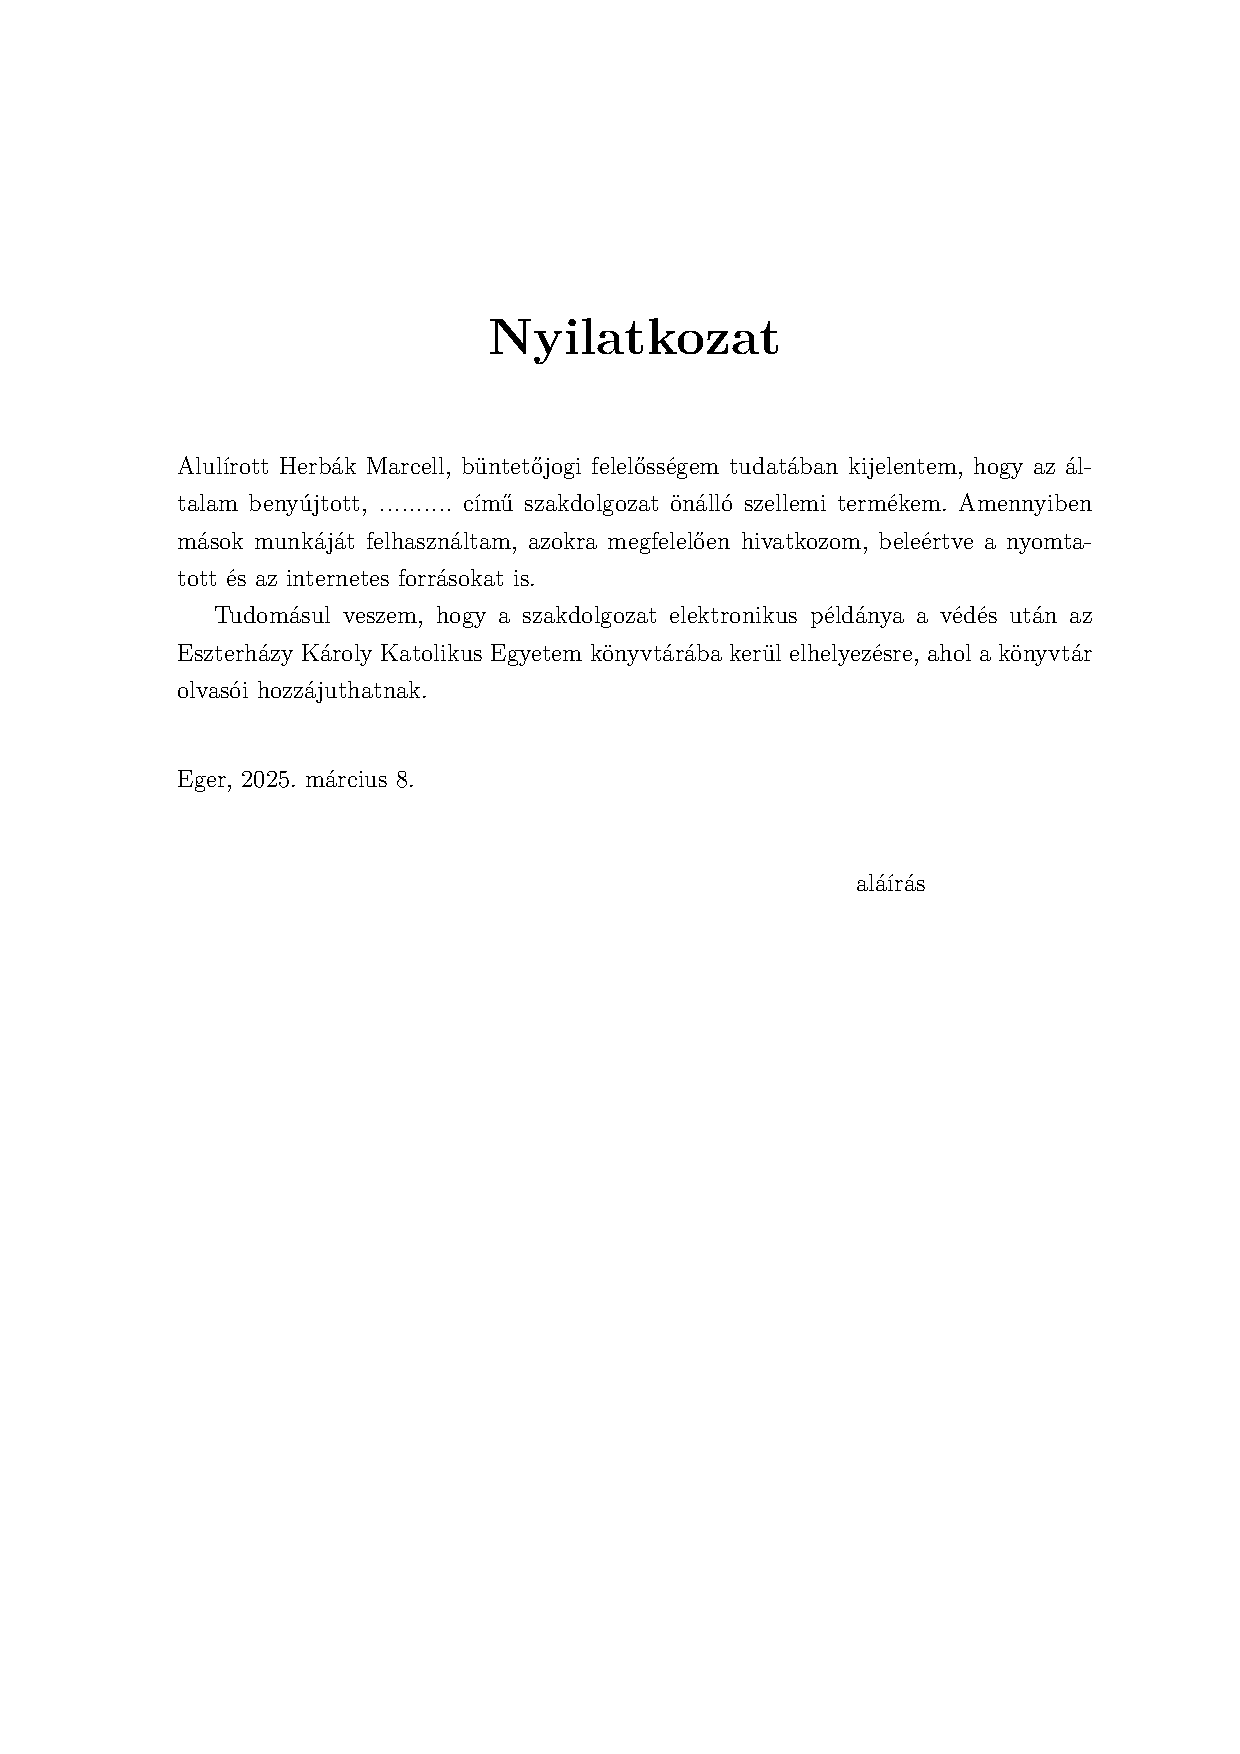
\includepdf{nyilatkozat/nyilatkozat.pdf}
\end{document}